\section{Tecniche per AI}
\begin{figure}[H]
    \centering
    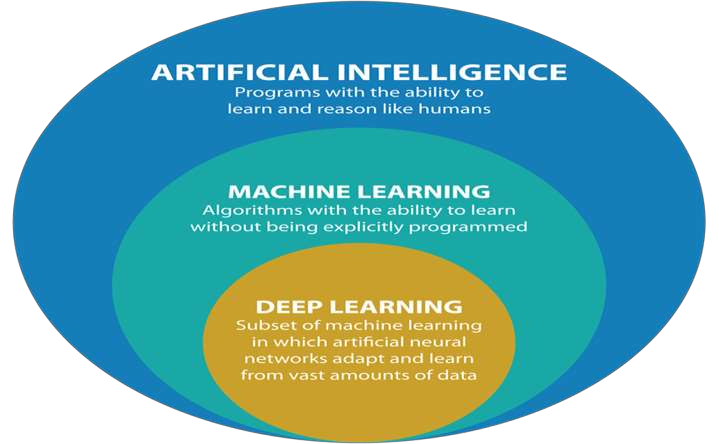
\includegraphics[width=0.5\linewidth]{imgs/12 - campi dell'ai}
    \caption{Branche della AI}
    \label{fig:campi_ai}
\end{figure}

Attualmente la AI si occupa di:
\begin{itemize}
    \item identificazione di modelli
    \item idedntificazioni algoritmi
\end{itemize}


\subsection{Costruzione di una IA}
\subsubsection{Conoscenza}
Conoscenza come:
\begin{itemize}
    \item informazioni(nozioni)
    \item conoscenza(cultura, dottrina)
    \item competenza(abilità, tecnica)
\end{itemize}

L'esperienza può venire sia da esperienze dirette che indirette.

Nei computer la conoscenza non è strettamente legata all'informazione, moli di dati non forniscono 
alcuna informazione.

\textbf{La conoscenza è informazione disponibile per un'azione razionale.}
Però non sempre una sceltarazionale è legata all'inferenza e viceversa.

\subsubsection{Agire razionale}
Gli individui agiscono sulla conoscenza e sulle percezioni del mondo attraverso ragionamento:
\begin{itemize}
    \item deduttivo: dalla premessa alla conclusion
    \item abduttivo: dagli effetti alle possibili cause
    \item induttivo: da fatti specifici a regole generali
\end{itemize}
per produrre nuova conoscenza.

\subsubsection{Due approcci differenti}
\begin{itemize}
    \item top down o simbolico
    La conoscenza è rappresentata da simboli. Vengono utilizzate la
    logica e la capacità di fare inferenze
    \item bottom up o subsimbolico
    Non esiste una rappresentazione esplicita della conoscenza.
    Vengono utilizzate reti neurali, approcci evolutivi, ecc
\end{itemize}

\begin{figure}[H]
    \centering
    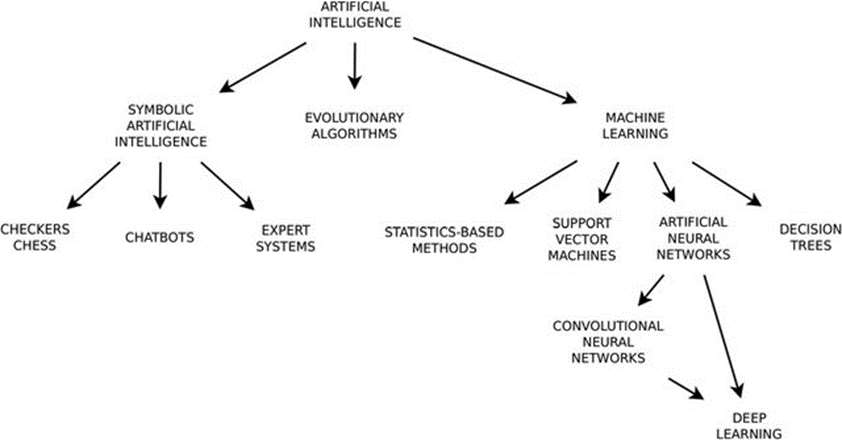
\includegraphics[width=0.8\linewidth]{imgs/13 - ai}
    \caption{Tecniche per AI}
    \label{fig:ai_tecniche}
\end{figure}

\subsection{Approccio simbolico}
Alla AI viene fornito una descrizione del dominio in linguaggio formale, per attingere
a questa base di conoscenza e inferire nuova conoscenza(o azioni da intraprendere).

\subsubsection{Logica}
La logica fornisce strumenti formali per:
\begin{itemize}
    \item Esprimere inferenze
    \item dedurre le conseguenze
    \item studiare la verità o la falsità
    \item stabilire la coerenza e la validità
\end{itemize}


La logica si basa sul ragionamento deduttivo.
In logica, la conoscenza iniziale è indicata come assiomi. Le nuove
conoscenze derivate dagli assiomi sono chiamate teoremi.

Per inferire nuovi teoremi si usa la \textbf{regola di inferenza}.(usando il simbolo "$\Rightarrow)$")

Esempio:
$A$ è vero, $B$ è vero $\Rightarrow$ C è vero.

In generale, in logica si studia la relazione tra le formule di un sistema logico-simbolico
in cui:
\begin{itemize}
    \item il linguaggio delle formule è definito con precisione
    \item il significato delle formule è stabilito in modo univoco
\end{itemize}

La logica moderna ha il compito si rappresentare in modo formale la corrispondenza tra espressioni
linguistiche e significato inteso.
Ls formalizzazione(astrazione) è una sorta di compressione delle informazioni, con ampia
perdita di dettaglio e guadagno di precisione.

\subsection{Logica proposizionale}
\subsubsection{La base}
La \textbf{logica} è un linguaggio formale per rappresentare informazioni e dedurre conclusioni,
la \textbf{sintassi} definisce le proposizioni ammissibili dal linguaggio,
la \textbf{semantica} definisce il "significato" dell'asserzione.

\subsubsection{Implicazione}
\begin{equation*}
    KB \models \alpha
\end{equation*}

La conoscenza KB implica $\alpha$, se $\alpha$ è vera allora KB sono verificati.


\subsubsection{Sintassi logica proposizionale}
\begin{itemize}
    \item definisce frasi ammissibili
    \item le frasi atomiche sono fatte da un singolo simbolo
    \item questi simboli possono essere veri o falsi
    \item le frasi complesse sono un insieme di frasi semplici
\end{itemize}

Connettivi:
\begin{itemize}
    \item negazione con sengo -
    \item and $\wedge$
    \item or $\vee$
    \item implicazione $\Rightarrow$
    \item equivalenza $\Leftrightarrow$
\end{itemize}

\subsubsection{Semantica logica proposizionale}
\begin{itemize}
    \item la semantica definisce le regole per determinare la verità di una frase rispetto al modello
    \item nella logica proposizionale, il modello fissa la verità
    \item le frasi sono costrutite dalle frasi atomiche e dai 5 connettivi
\end{itemize}

Bisogna usare delle tabelle di verità.

\subsubsection{Limiti della logica proposizionale}
Troppo semplice, una merda.

\subsection{AI e ontologie, tecnologie semantiche}
\subsubsection{Logica descrittiva e ontologie}
i metodi semantici e le reti semantiche usano sitemi di logica descrittiva, adatta al ragionamento automatico.
\textbf{In AI, l'ontologia è una descrizione formale esplicita di un dominio di interesse.}


Quindi un ontologia è costituita da:
\begin{itemize}
    \item classi(concetti generali del dominio di interesse)
    \item relazioni tra queste classi
    \item proprietà assegnate a ciascun concetto, che ne descrivono vari tipi di attributi o proprietà
    \item restrizioni sulle proprietà
\end{itemize}

A partire dalle classi di ontologia, è possibile definire delle istanze, che rappresentano specifici oggetti
del mondo reale.

Knowledge base = Ontologia + insieme delle istanze delle classi.

Esistono ontologie specifiche(inerenti al dominio di applicazione) e generali.

Le ontologie organizzano tutti gli elementi della realtà in una gerarchia di categorie,
gli elementi padre passano i loro attributi ai figli(come nella programmazione a classi).

Esempio pizza:
\begin{figure}[H]
    \centering
    \includegraphics[width=0.8\linewidth]{imgs/14 - pizza ontologia eredità}
    \caption{Ontologia: Esempio della pizza}
    \label{fig:pizza}
\end{figure}

\subsubsection{Ontologia: termini ricorrenti}
\begin{itemize}
    \item Sussunzione: usata per creare gerarchie
    \item meronimia: descrive come si combinano i concetti
    \item vocabolario controllato: lista di termini numerati
    \item tassonomia: collezione di termini
    \item thesaurus: rete di termini
\end{itemize}
\subsubsection{Ontologia: operazioni tipiche}
\begin{itemize}
    \item costruire un modello ontologico
    \item eseguire il mapping tra concetti
    \item unire in un modello le informazioni
\end{itemize}
\subsubsection{Vantaggi delle ontologie}
\begin{itemize}
    \item permette la rappresentazione esplicita di modelli semantici
    \item abilitano l'applicazione di strumnti capaci di ragionamento
    \item adattamento a contesti differenti
    \item capacità di modellare domini che evolvono
\end{itemize}

\subsubsection{Ontologie: limiti}
\begin{itemize}
    \item difficoltà di rappresentare il problema
    \item avere uno standard
\end{itemize}

\subsection{IA: approccio sub-simbolico}
L'apprendimento deriva dall'esperienza.

\subsubsection{Comportamenti emergenti}
Nei sistemi complessi si parla di \textbf{compotamenti emergenti}, osservabili quando
l'attenzione si sposta dal singolo individuo alla collettività.

Spesso non rispecchiano il comportamento previsto.

Si cerca di programmare i singoli elementi dotandoli di far tendere il collettivo verso una direzione.

Si lascia poi che il sistema si organizzi.

\subsubsection{Ragionamento e apprendimento}
Il sistema intelligente deve saper ragionare e di acquisire nuova conoscenza in autonomia.

L'apprendimento è fondamentale per:
\begin{itemize}
    \item risolvere nuovi problemi
    \item non ripetere errori
    \item risolvere problemi in maniera più efficiente
    \item avere autonomia e adattarsi
\end{itemize}

\subsubsection{Apprendimento induttivo}
dato un insieme di esempi(campioni) di f, definsci una funzione h(ipotesi) che approssima f.

Si cerca di generalizzare le infromazioni per prevedere altre siteuazioni.

\subsubsection{Apprendimento da esempi}
Con l'apprendimento induttivo, gli esempi possono essere costruiti da:
\begin{itemize}
    \item descrizioni(pattern) di un'istanza di un fenomeno/problema da risolvere.
    \item insieme di coppie di dati
\end{itemize}

Per ottenere un buon esempio da dare in apprendimento, l'esempio deve essere rappresentativo del problema.

Abbastanza esempi??

\subsection{Inferenza in IA}
\subsubsection{Sistemi esperti}
Un sistema esperto è un sistema basato su regole di produzione che, a partire da alcuni dati, cerca
di dimostrare un'ipotesi.

\begin{enumerate}
    \item IF Meteo=‘Soleggiato’ AND Umidità=‘Bassa’ THEN Gioco
    \item IF Meteo=‘Soleggiato’ AND Umidità=‘Alta’ THEN Non Gioco
    \item IF Meteo= ‘Pioggia’ AND Vento = VERO THEN Non Gioco
    \item IF Meteo= ‘Pioggia’ AND Vento = FALSO THEN Gioco
    \item IF Meteo= ‘Nuvoloso’ THEN Gioco
    \item ELSE Gioco
\end{enumerate}

Prende una decisione sui fatti disponibili.

\subsubsection{Alberi decisionali}
Si può costruire un albero decisionale da una serie di esempi.

\subsubsection{Learnign = infering + memorizing}
durante l'apprendimento se un dato risulta utile, viene memorizzato.

Le inferenze possono essere deduttive o induttive.

Le inferenze possono essere divise in inferenze forti(conclusioni) o deboli(contingenti).

\subsection{Black box AI \& explainable AI}
I sitemi di ML possono funzioanre in questi due modi.


\subsubsection{Reti neurali artificiali: deep learning}
\begin{itemize}
    \item difficoltà a generalizzare
    \item scarso capacità di inferenza e gestione del agionamento logico
    \item difficile spiegare il loro comportamento
    \item difficoltà a ditinguere correzioni e causa-effetto
\end{itemize}

Explainable AI (XAI) studia il motivo per cui è stata presa una decisione
dall’AI in modo che i modelli di AI possano essere più interpretabili per gli
utenti umani e consentire loro di capire perché il sistema è arrivato a una
decisione specifica.

XAI aiuta a portare trasparenza nell'IA, rendendo potenzialmente possibile
aprire la scatola nera.

\subsubsection{Indagare un sistema AI}

Un primo livello di indagine riguarda l’Interpretability (interpretabilità)
cioè la possibilità di mettere in relazione causale i dati in ingresso con
quelli in uscita.

Consiste nel fornire una spiegazione del perché il modello ha fatto una
certa scelta o ha fornito una determinata previsione (WHAT).

Capire l'algoritmo.

Un secondo livello è inerente alla capacità di spiegare in termini comprensibili su come il modello sia
arrivato ad una conclusione.


Alcuni approcci sono:
\begin{itemize}
    \item spiegazione testuale
    \item esempi
    \item semplificazione del modello
    \item visualizzazione
    \item spiegazione locale: spiegare sotto-porzioni del sistema
    \item features rilevanti
\end{itemize}





















